\documentclass[crop,tikz]{standalone}

\usepackage{tikz}
\usetikzlibrary{automata, positioning, arrows}
\begin{document}
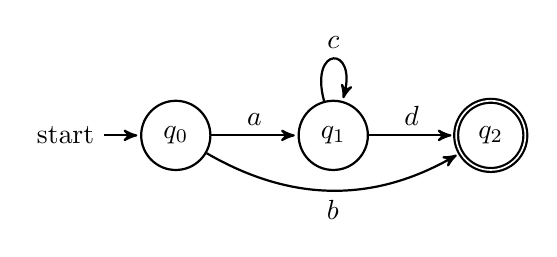
\begin{tikzpicture}[shorten >=1pt,node distance=2cm,>=stealth',thick]
\node[state, initial] (0) {$q_0$};
\node[state, right of=0] (1) {$q_1$};
\node[state, accepting, right of=1] (3) {$q_2$};
\draw[->] (0) edge[above] node{$a$} (1)
(0) edge[below, bend right, below=0.5] node{$b$} (3)
(1) edge[loop above, above] node{$c$} (1)
(1) edge[above] node{$d$} (3);
\end{tikzpicture}
\end{document}